
%%%%%%%%%%%%%%%%%%%%%%%%%%%%%%%%%%%%%%%%%%%%%%%%%%%
\section{Architecture}
\label{sec:Architecture}
%%%%%%%%%%%%%%%%%%%%%%%%%%%%%%%%%%%%%%%%%%%%%%%%%%%


We now present the architectural specifications of \ac{bard}. The CRISP-DM model was used as a baseline for representing data life cycle. \ac{bard} focuses on Data Quality (\textit{e.g.}: cleaning, annotation), Data Representation (\textit{e.g.}: anonymization, ciphering) and Data Processing (\textit{e.g.}: Computation on ciphertext).

The Data Quality step refers to the transformation of raw input data into a structured, consistent and, whenever possible, complete representation. An important aspect to mention in this step is that the data must be processed in plaintext by a trusted entity, meaning it is done by the owned of the data or an entity in which the owner of the data trusts and has explicit permission to perform the operations.
The Data Representation step refers to the protection of \ac{pii} contained in the data. This data should be integrated using privacy-preserving data integration techniques, data should be aggregated using anonymization techniques and data should be represented using either hashing techniques or homomorphic cryptosystems.
The Data Processing step is done in two different approaches. On one hand, \ac{smpc} techniques, such as \ac{gc} and \ac{he}, are performed over the data. On the other hand, \ac{ml} algorithms, adapted to work with hashed or encrypted data, are used in performing knowledge learning.

We now describe the internal structure that the project aims to provide.
As stated in the objectives, the main goal of \ac{bard} is to produce a platform that will provide mechanisms so that companies can perform privacy-preserving computations for \ac{ml} algorithms, that are respectful of user privacy, and comply with the legislation. A representation of the internal structure of that platform is described by the following components: 
\begin{itemize}
	\item \textbf{A dataset} to train the \ac{ml} algorithm, or the values representing the already trained algorithm.
	\item \textbf{A sample} or a set of samples that represent the input of the ``user'', to be predicted.
	\item \textbf{A prediction algorithm} that depends on the \ac{ml} algorithm and the privacy-preserving technique chosen.
	\item \textbf{A set of toolkits} for each of the techniques used.
\end{itemize}

These components altogether allow the user of the platform to perform privacy-preserving \ac{ml} over data of his own choosing.
In figure \ref{fig:bard-architecture}, we present the architecture for \ac{bard}, showing the components and steps that were taken in the design and implementation of the platform.

\begin{figure}[H]
\centering
\label{fig:bard-architecture}
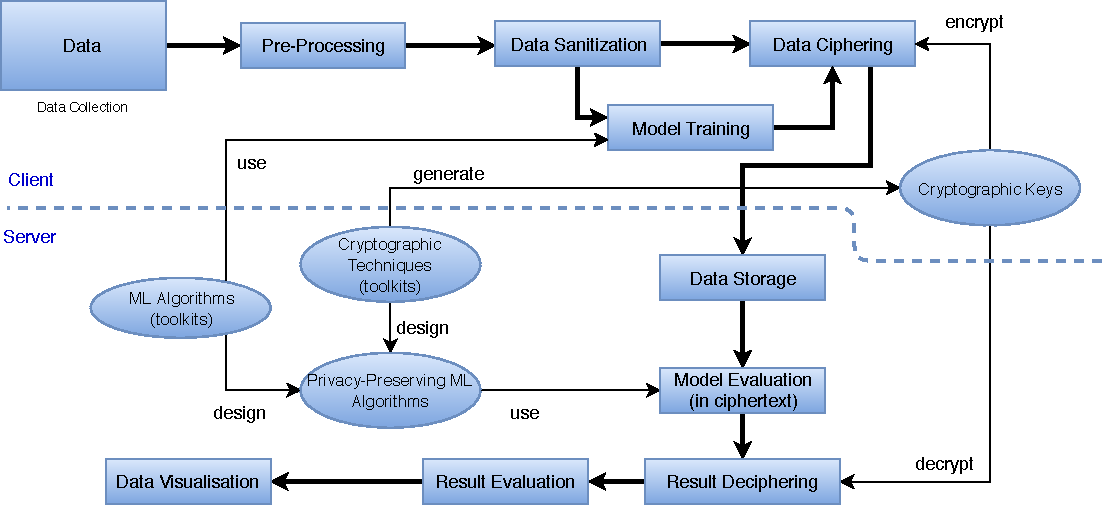
\includegraphics[width=1\textwidth]{images/BARDArchitecture.pdf}
\caption{Platform architecture for \acs{bard}.}
\end{figure}

%%%%%%%%%%%%%%%%%%%%%%%%%%%%%%%%%%%%%%%%%%%%%%%%%%%
\section{Our Contributions to \acs{bard}}
\label{sec:MyContributions}
%%%%%%%%%%%%%%%%%%%%%%%%%%%%%%%%%%%%%%%%%%%%%%%%%%%

It is important to mention that, in the following chapters of this thesis, we will present results that were not done by us. Since this thesis is part of a larger project developed in Altran, the implementation was done by a team of developers. As so, some results are presented for completeness of the solution, but were not obtained by us. Those results are the ones obtained using \ac{he}.

Our contributions to the project are then the development of a solution using the toolkit VIPP for privacy-preserving computations using \ac{gc}. This includes the development of the baseline part of the implementation, the expanded algorithms, the testing of the various toolkits and the actual development of the final solution with \ac{gc}. Throughout the rest of the document we will highlight the parts that were not developed by us. 

